%
% WirbelringKanone.tex -- praktische Applikation und anleitung zum Bau einer Wirbelringkanone
%
% !TEX root = ../../buch.tex
% !TEX encoding = UTF-8
%
\section{Praktische Applikation und Versuche für zu Hause}

Um dieses Thema passend abzuschliessen, zeigen wir im folgenden Abschnitt eine Möglichkeit Wirbelringe zu erzeugen.
Es gibt natürlich diverse Möglichkeiten, einen Wirbelring zu erzeugen. 
Hier zeigen wir einen Ansatz, welcher möglichst einfach und nachbaubar ist.

\subsection{Bau}

\begin{figure}
\centering
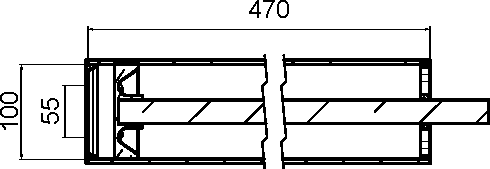
\includegraphics[width=0.8\textwidth]{papers/wirbelringe/fig/zeichnung.pdf}
\caption{Zeichnung und Masse der Wirbelringkanone \cite{Wirbelringe:3D_modelle} \label{Wirbelringe:fig:zeichnung}}
\end{figure}
Für den Bau wird ein (oder Zugang zu einem) 3D-Drucker, \diameter 100 PVC Abflussrohr und eine Möglichkeit, Rauch zu erzeugen, um die Wirbelringe sichtbar zu machen. 
Es müssen lediglich alle Teile 3D gedruckt werden (siehe \cite{Wirbelringe:3D_modelle}) und diese mit einem PVC Kleber fixiert werden. 
Die Konstruktion ist in Abbildung \ref{Wirbelringe:fig:zeichnung} dargestellt.

\subsection{Versuche}

\subsubsection{Wirbelringe erzeugen\label{Wirbelringe:wirbelringeerzeugen}}

Um nun mit dieser Wirbelringkanone Wirbelringe zu erzeugen, muss der Kolben vollständig zurückgezogen werden und die entstehende Kavität mit möglichst dichtem Rauch oder Nebel gefüllt werden.
Für langanhaltende Wirbelringe sollte ein möglichst windstiller Durchführungsort gewählt werden.
Zum Erzeugen von Wirbelringen muss lediglich der Kolben nach vorne bewegt werden.
Aus Gleichung \eqref{Wirbelringe:eq:naeherungZirkulation} ist ersichtlich, dass sowohl die Länge als auch die Geschwindigkeit, die der Kolben bewegt wird relevant ist.
Daher brauch es eventuell mehrere Versuche, damit ein Wirbelring entsteht.
Kurze, ruckartige Bewegungen sind dabei langen, langsamen Bewegungen vorzuziehen.

\subsubsection{Wirbelringe teilen}

Aus Abschnitt \ref{Wirbelringe:Grenzflaechen} ist bekannt, dass Wirbel nur auf Grenzflächen oder sich selbst enden können. 
Um das bei einem Wirbelring aufzuzeigen, kann ein Wirbelring „gespalten“ werden. 
Ein Wirbelring soll dazu gebracht werden, die Grenzflächen von sich selbst auf etwas anderes, zum Beispiel ein Tisch, zu ändern. 
Mithilfe einer Kante, die wie eine Klinge funktioniert, kann der Wirbelring geschnitten und so umgelenkt werden, dass der jetzige Wirbelfaden sich weiter bewegt. 
Dieser Versuch ist in Abbildung \ref{Wirbelringe:fig:wirbelringversuch} dargestellt und beinhaltet folgenden Ablauf:

\begin{figure}
    \centering
    \subfigure[\label{Wirbelringe:fig:versuch_moment_1}]{
        %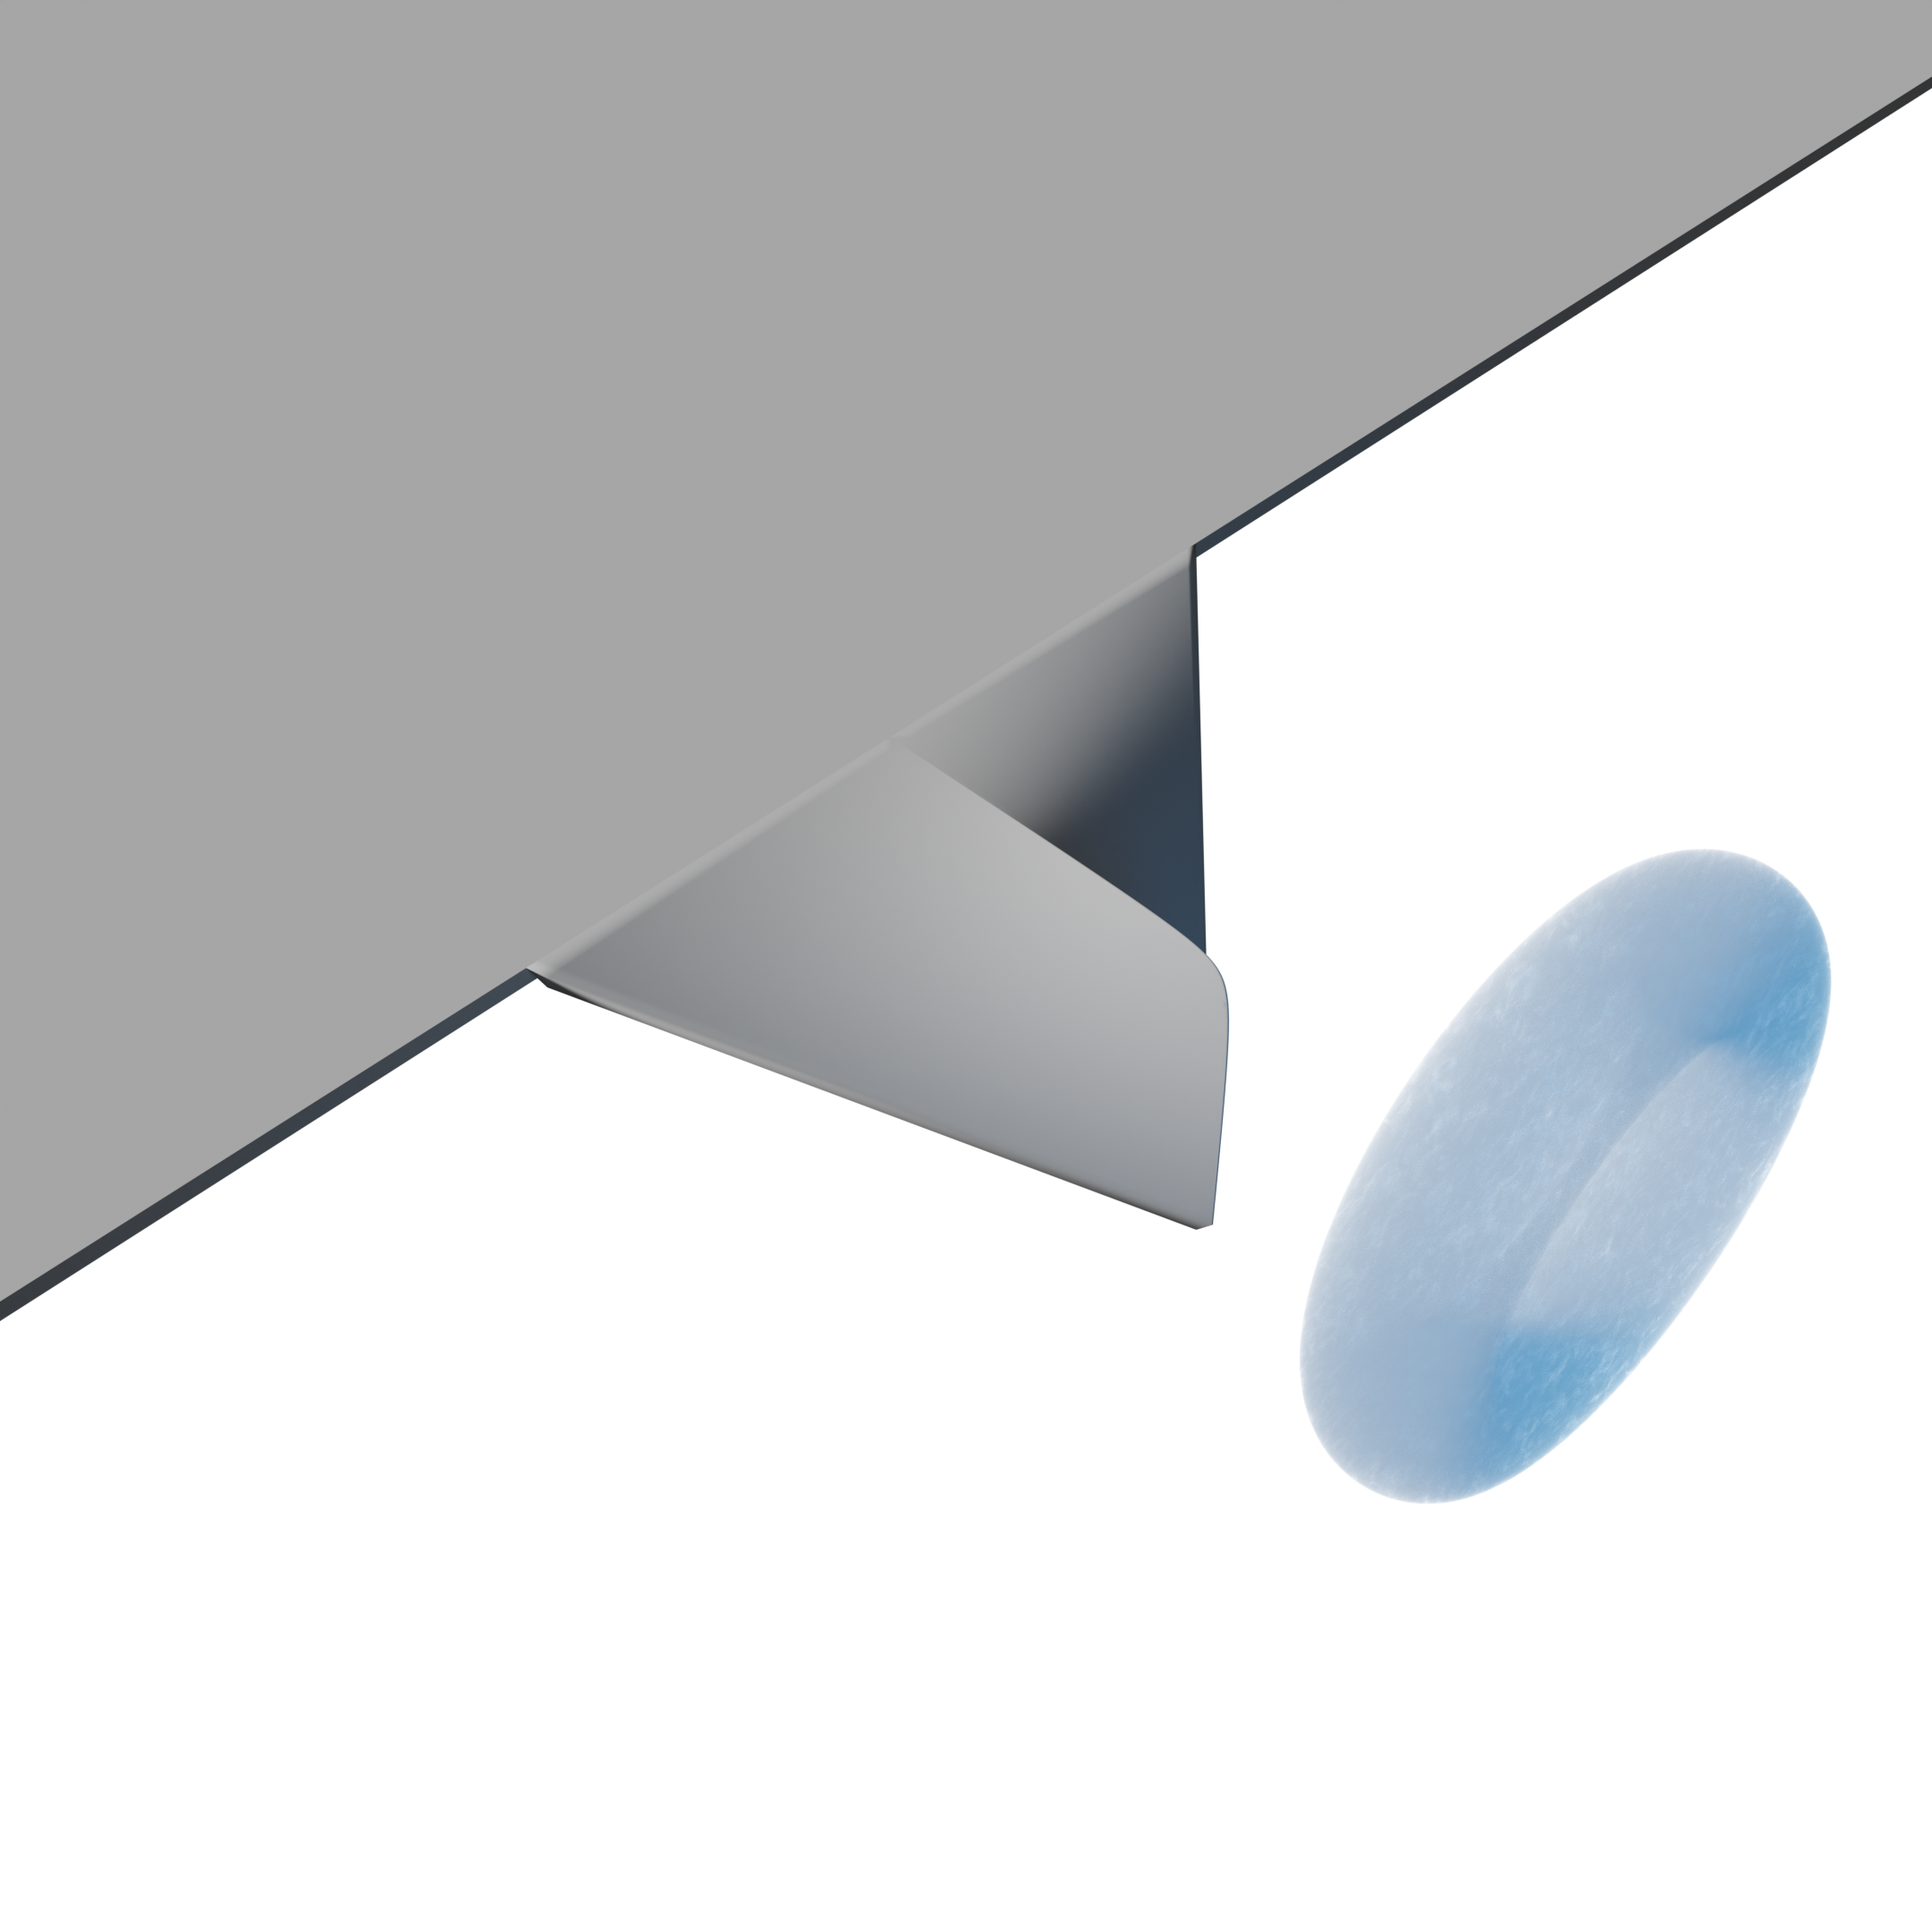
\includegraphics[width=0.3\textwidth]{papers/wirbelringe/fig/versuch_moment_1.png}
        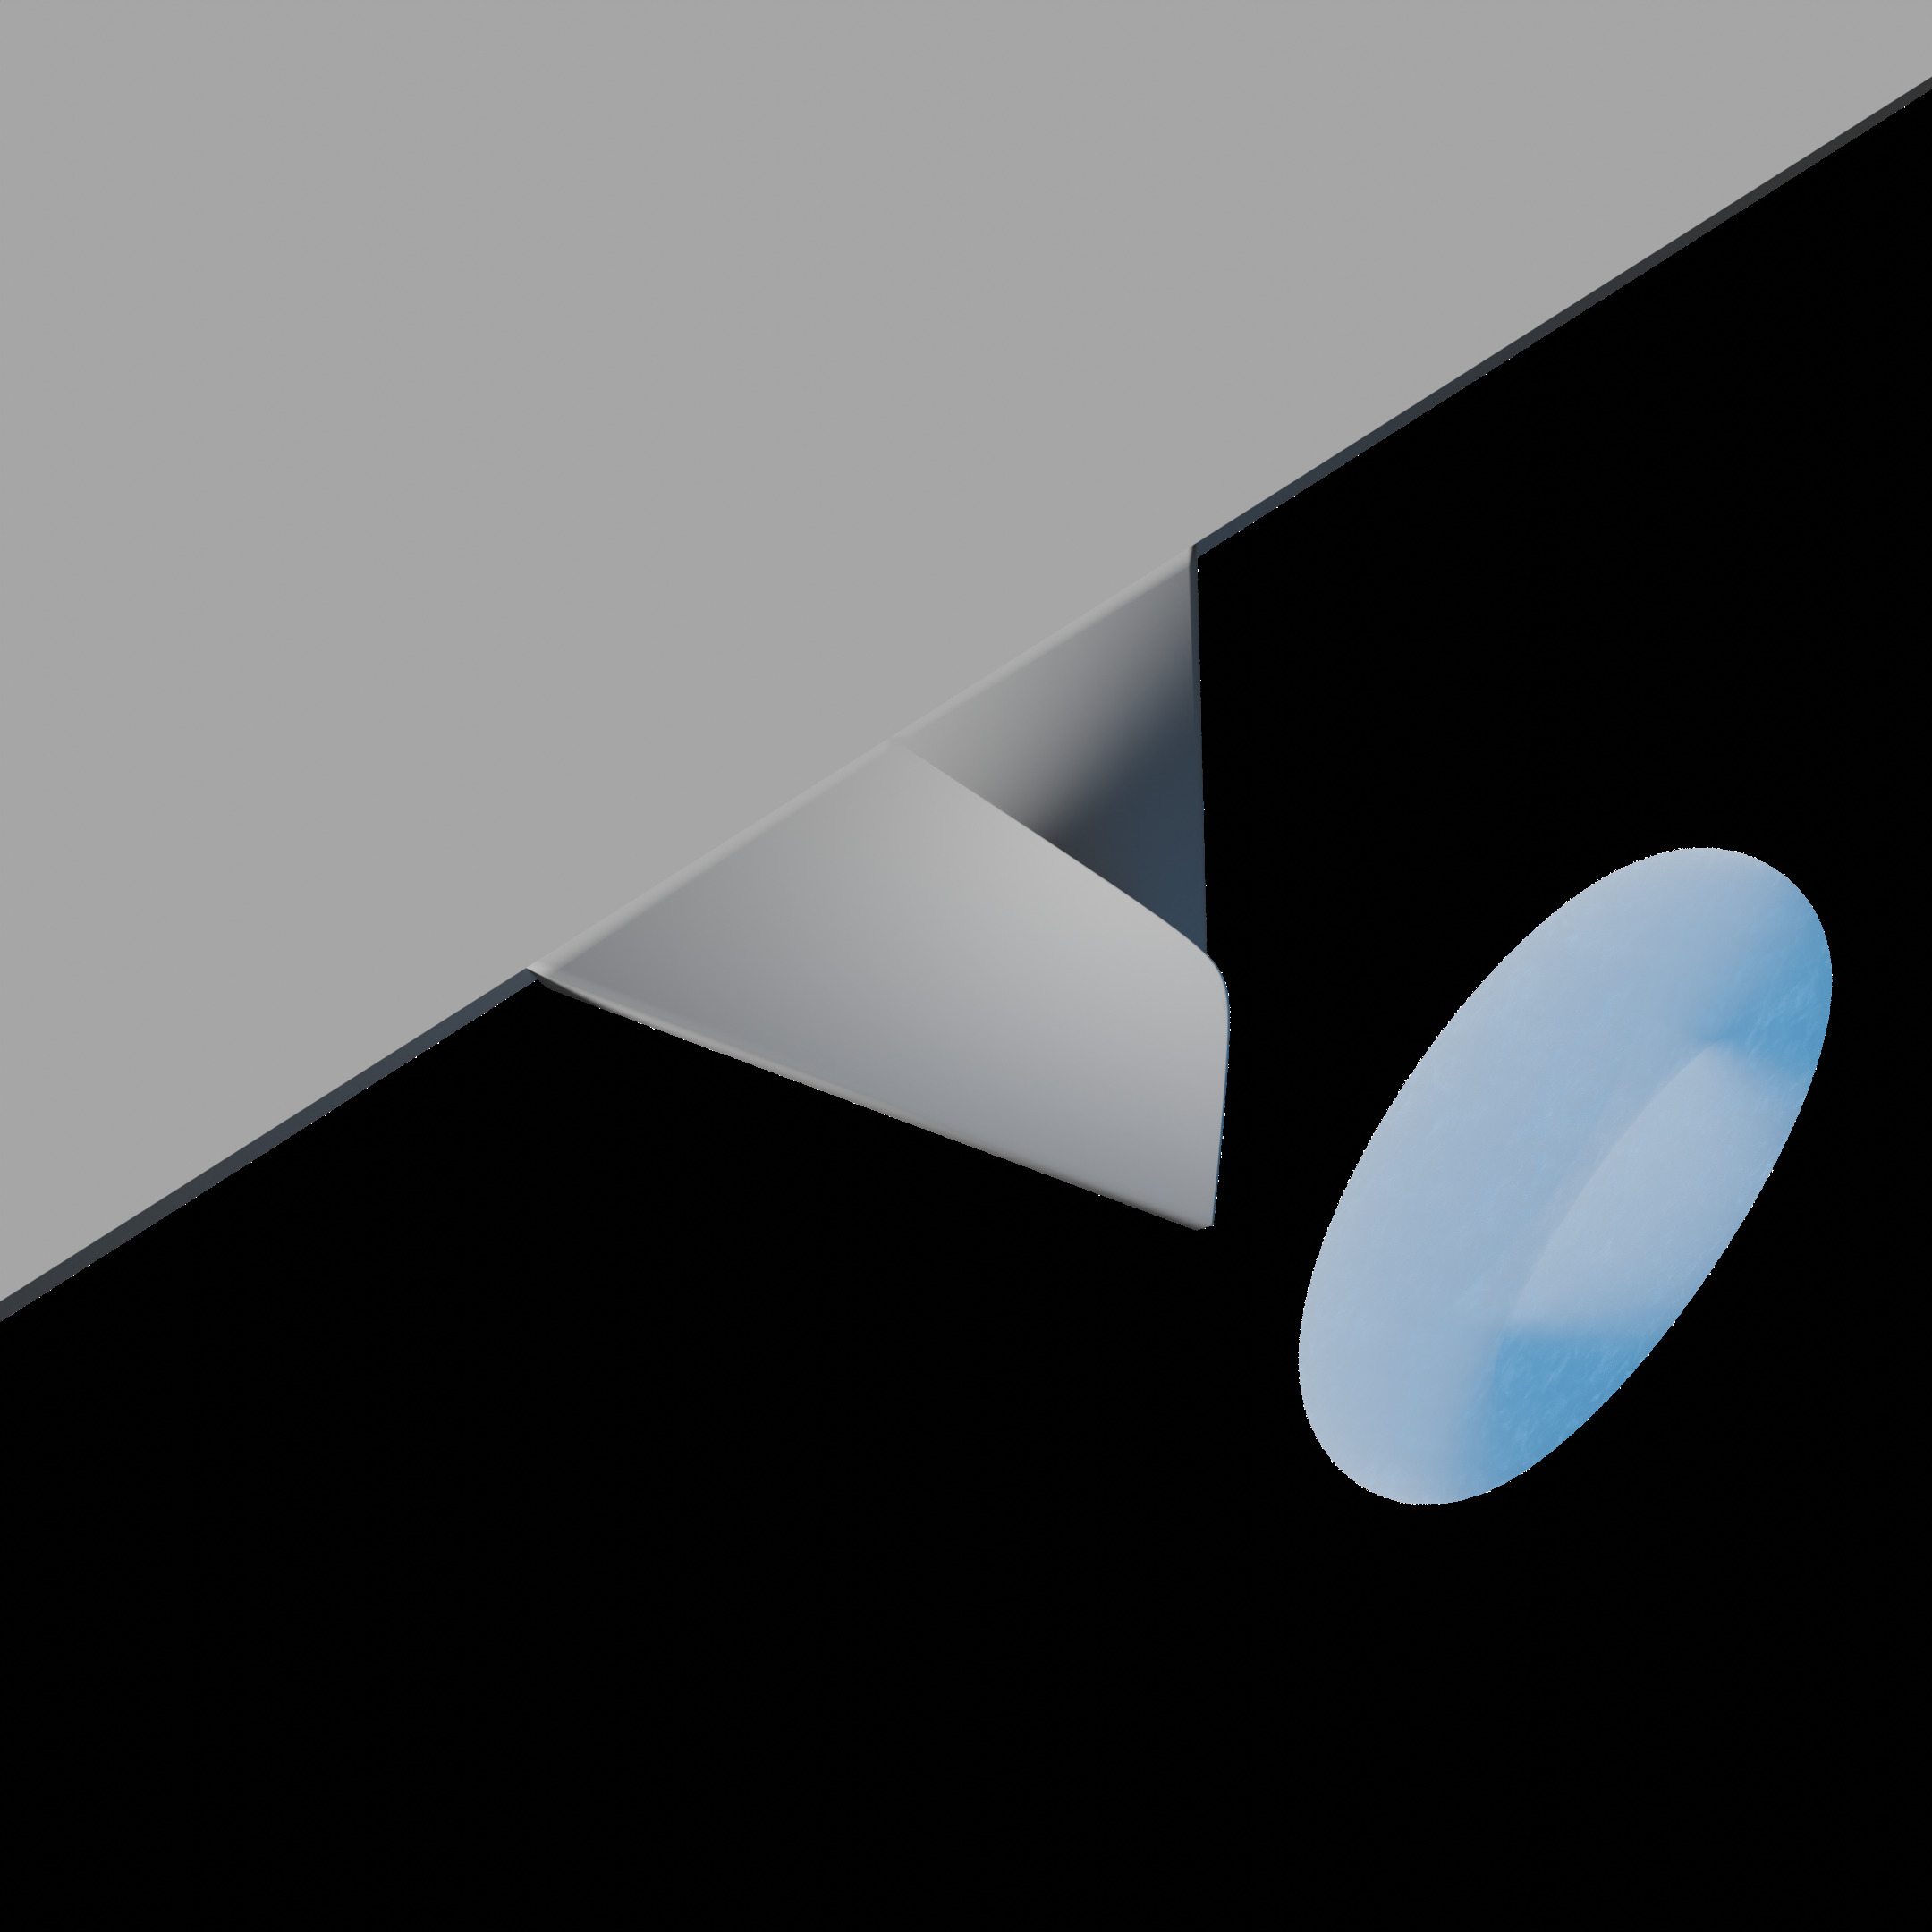
\includegraphics[width=0.3\textwidth]{papers/wirbelringe/fig/versuch_moment_1.jpg}
    }\hfill
    \subfigure[\label{Wirbelringe:fig:versuch_moment_2}]{
        %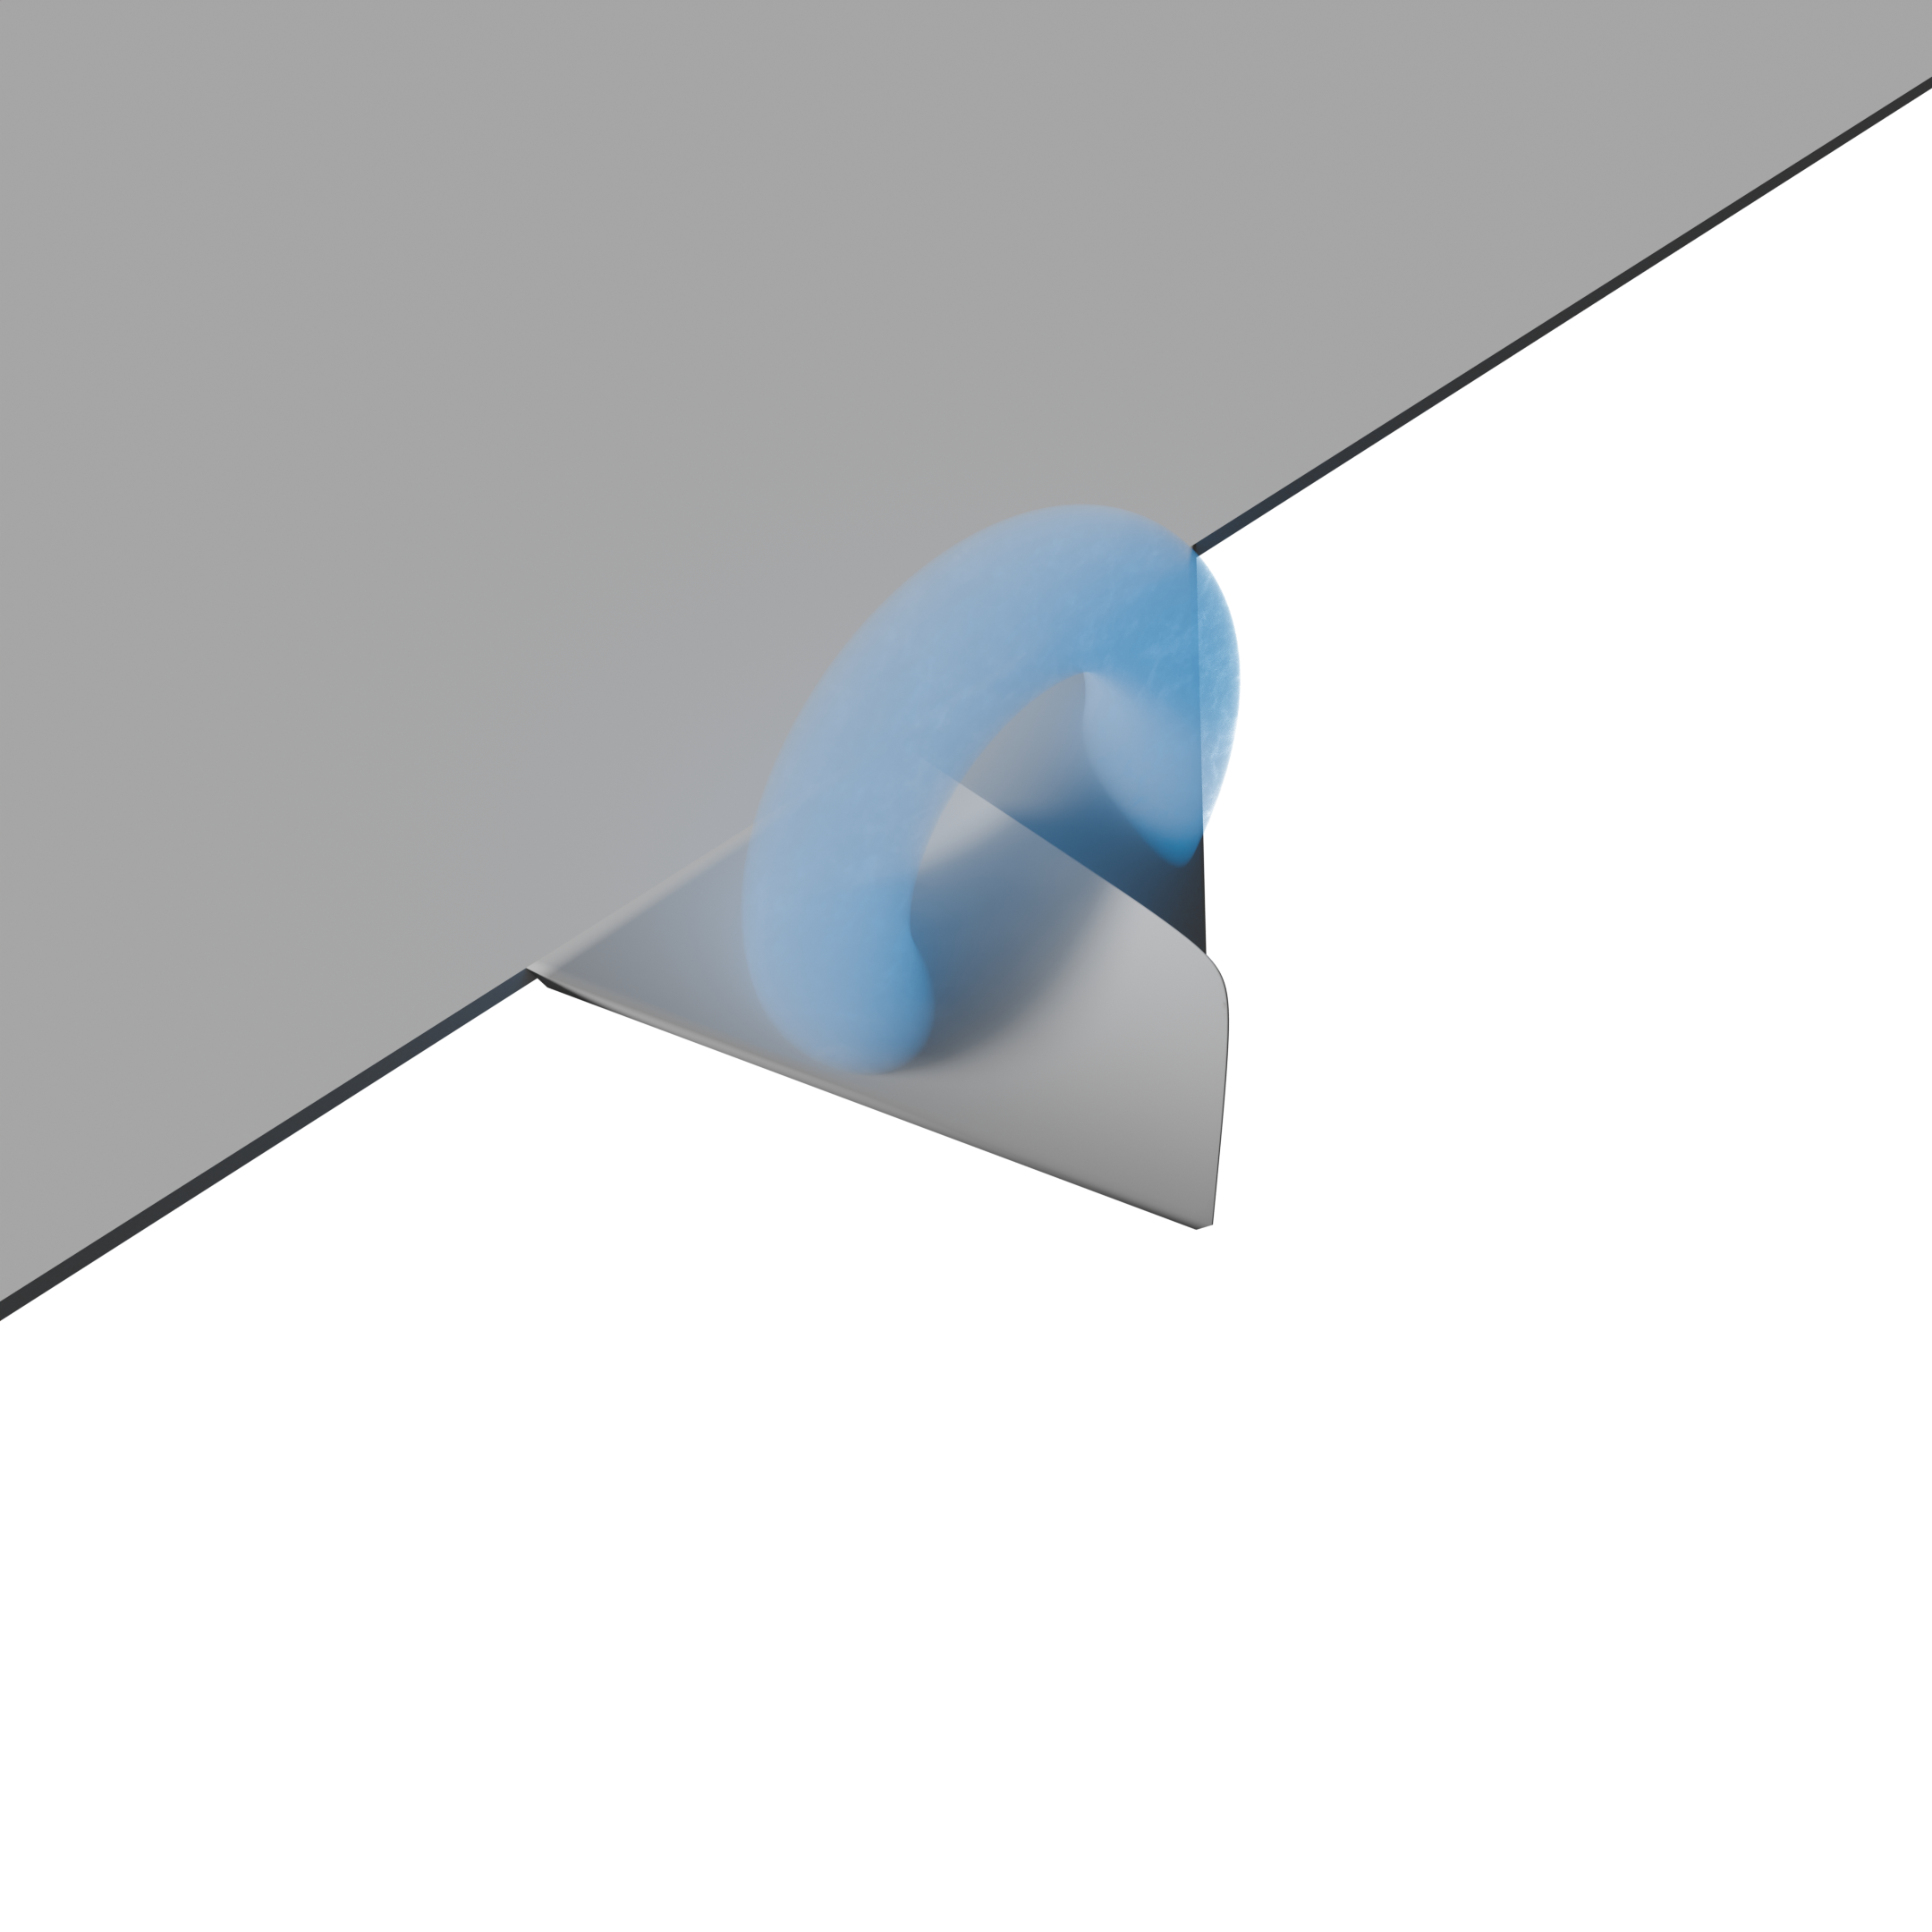
\includegraphics[width=0.3\textwidth]{papers/wirbelringe/fig/versuch_moment_2.png}
        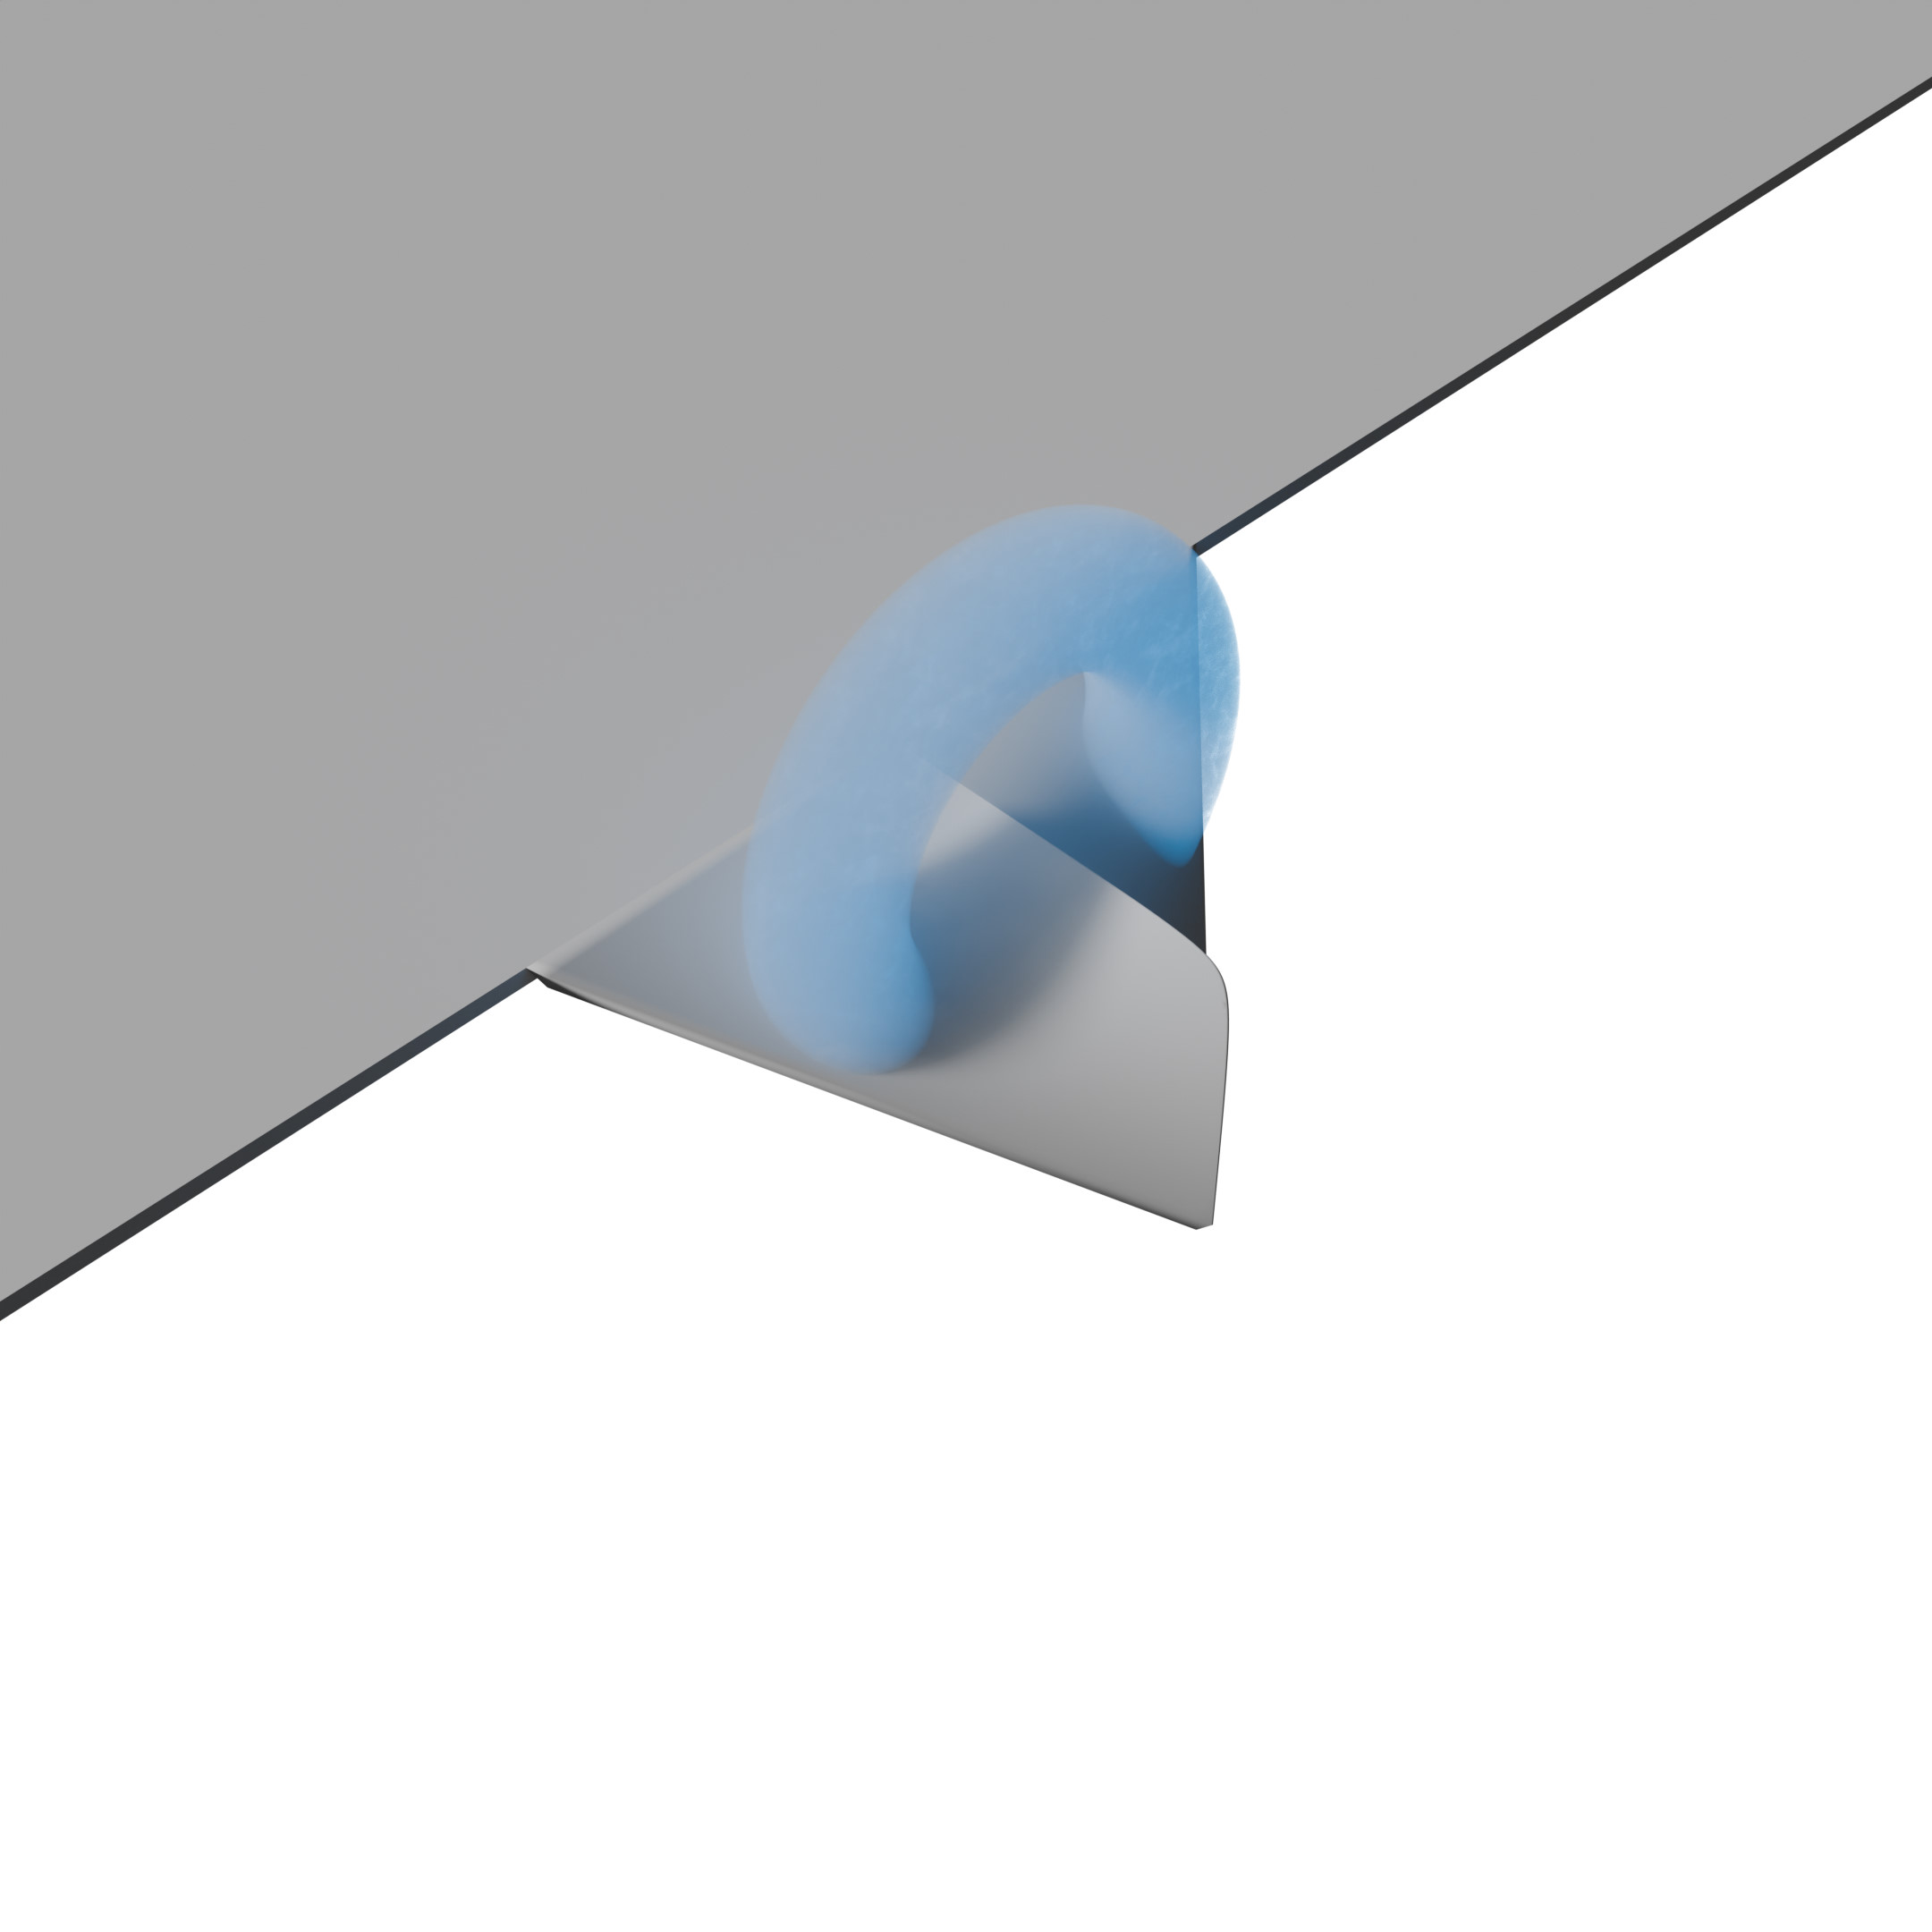
\includegraphics[width=0.3\textwidth]{papers/wirbelringe/fig/versuch_moment_2.jpg}
    }\hfill
    \subfigure[\label{Wirbelringe:fig:versuch_moment_3}]{
        %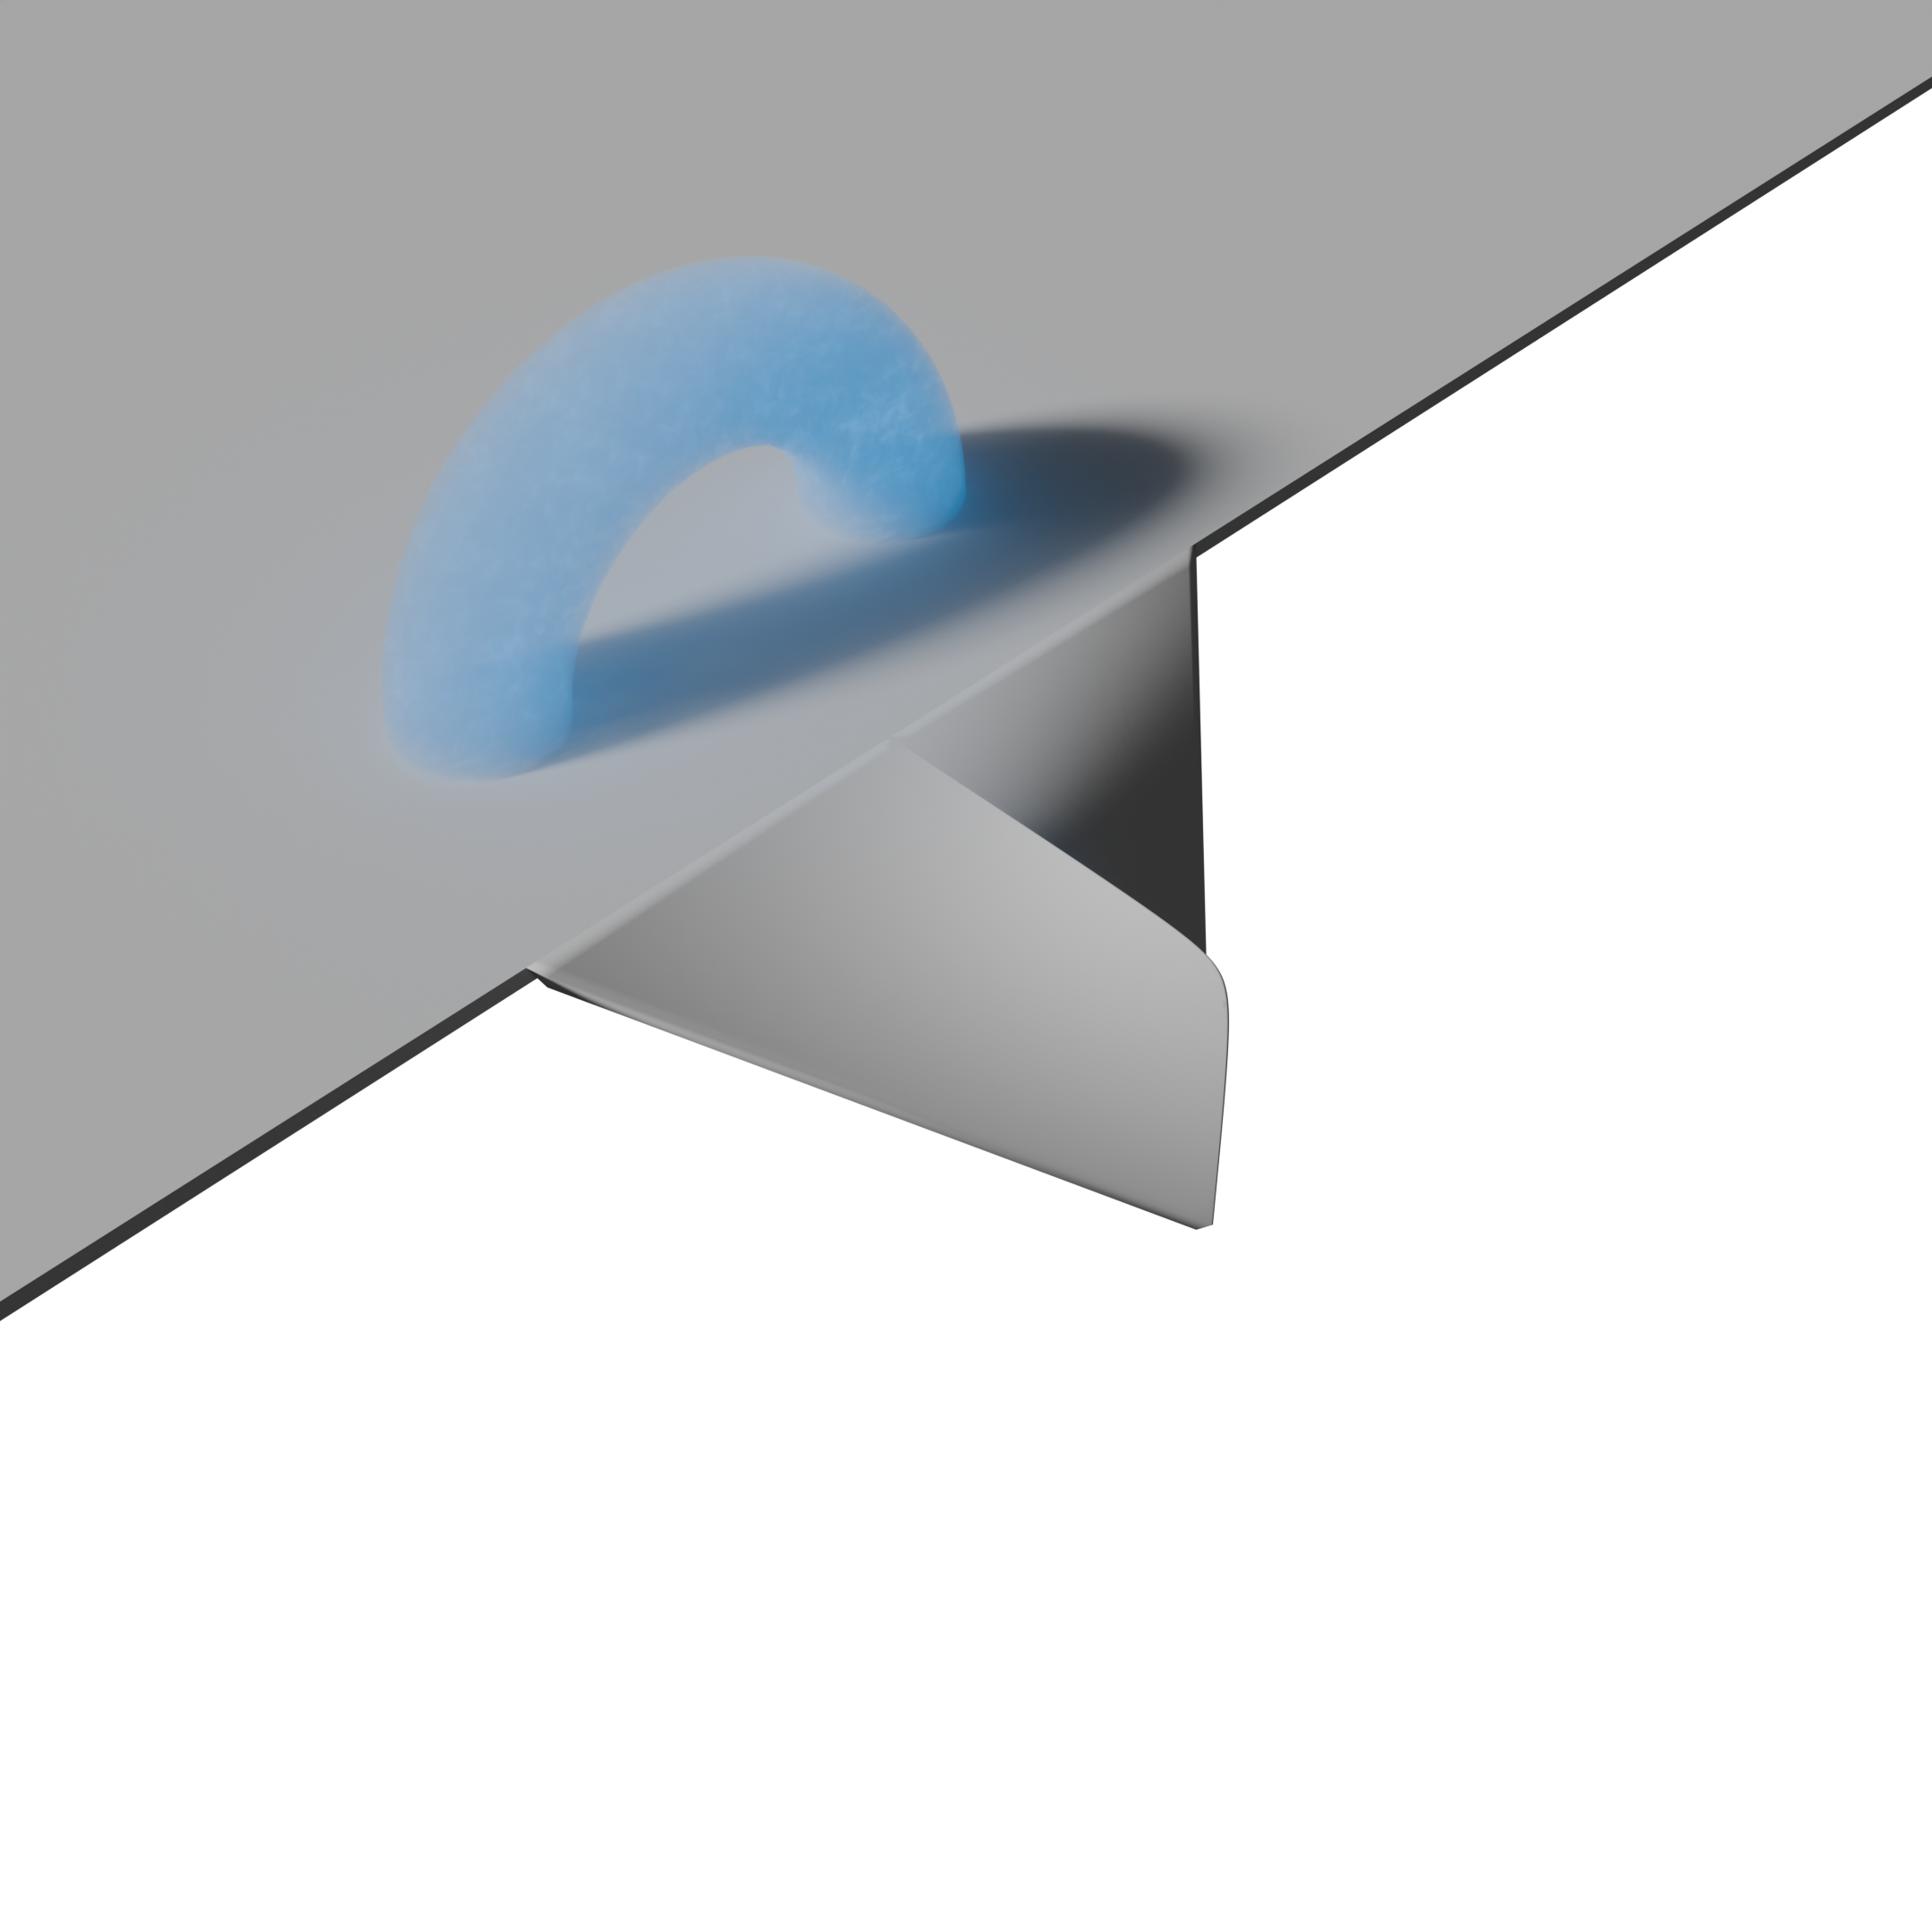
\includegraphics[width=0.3\textwidth]{papers/wirbelringe/fig/versuch_moment_3.png}
        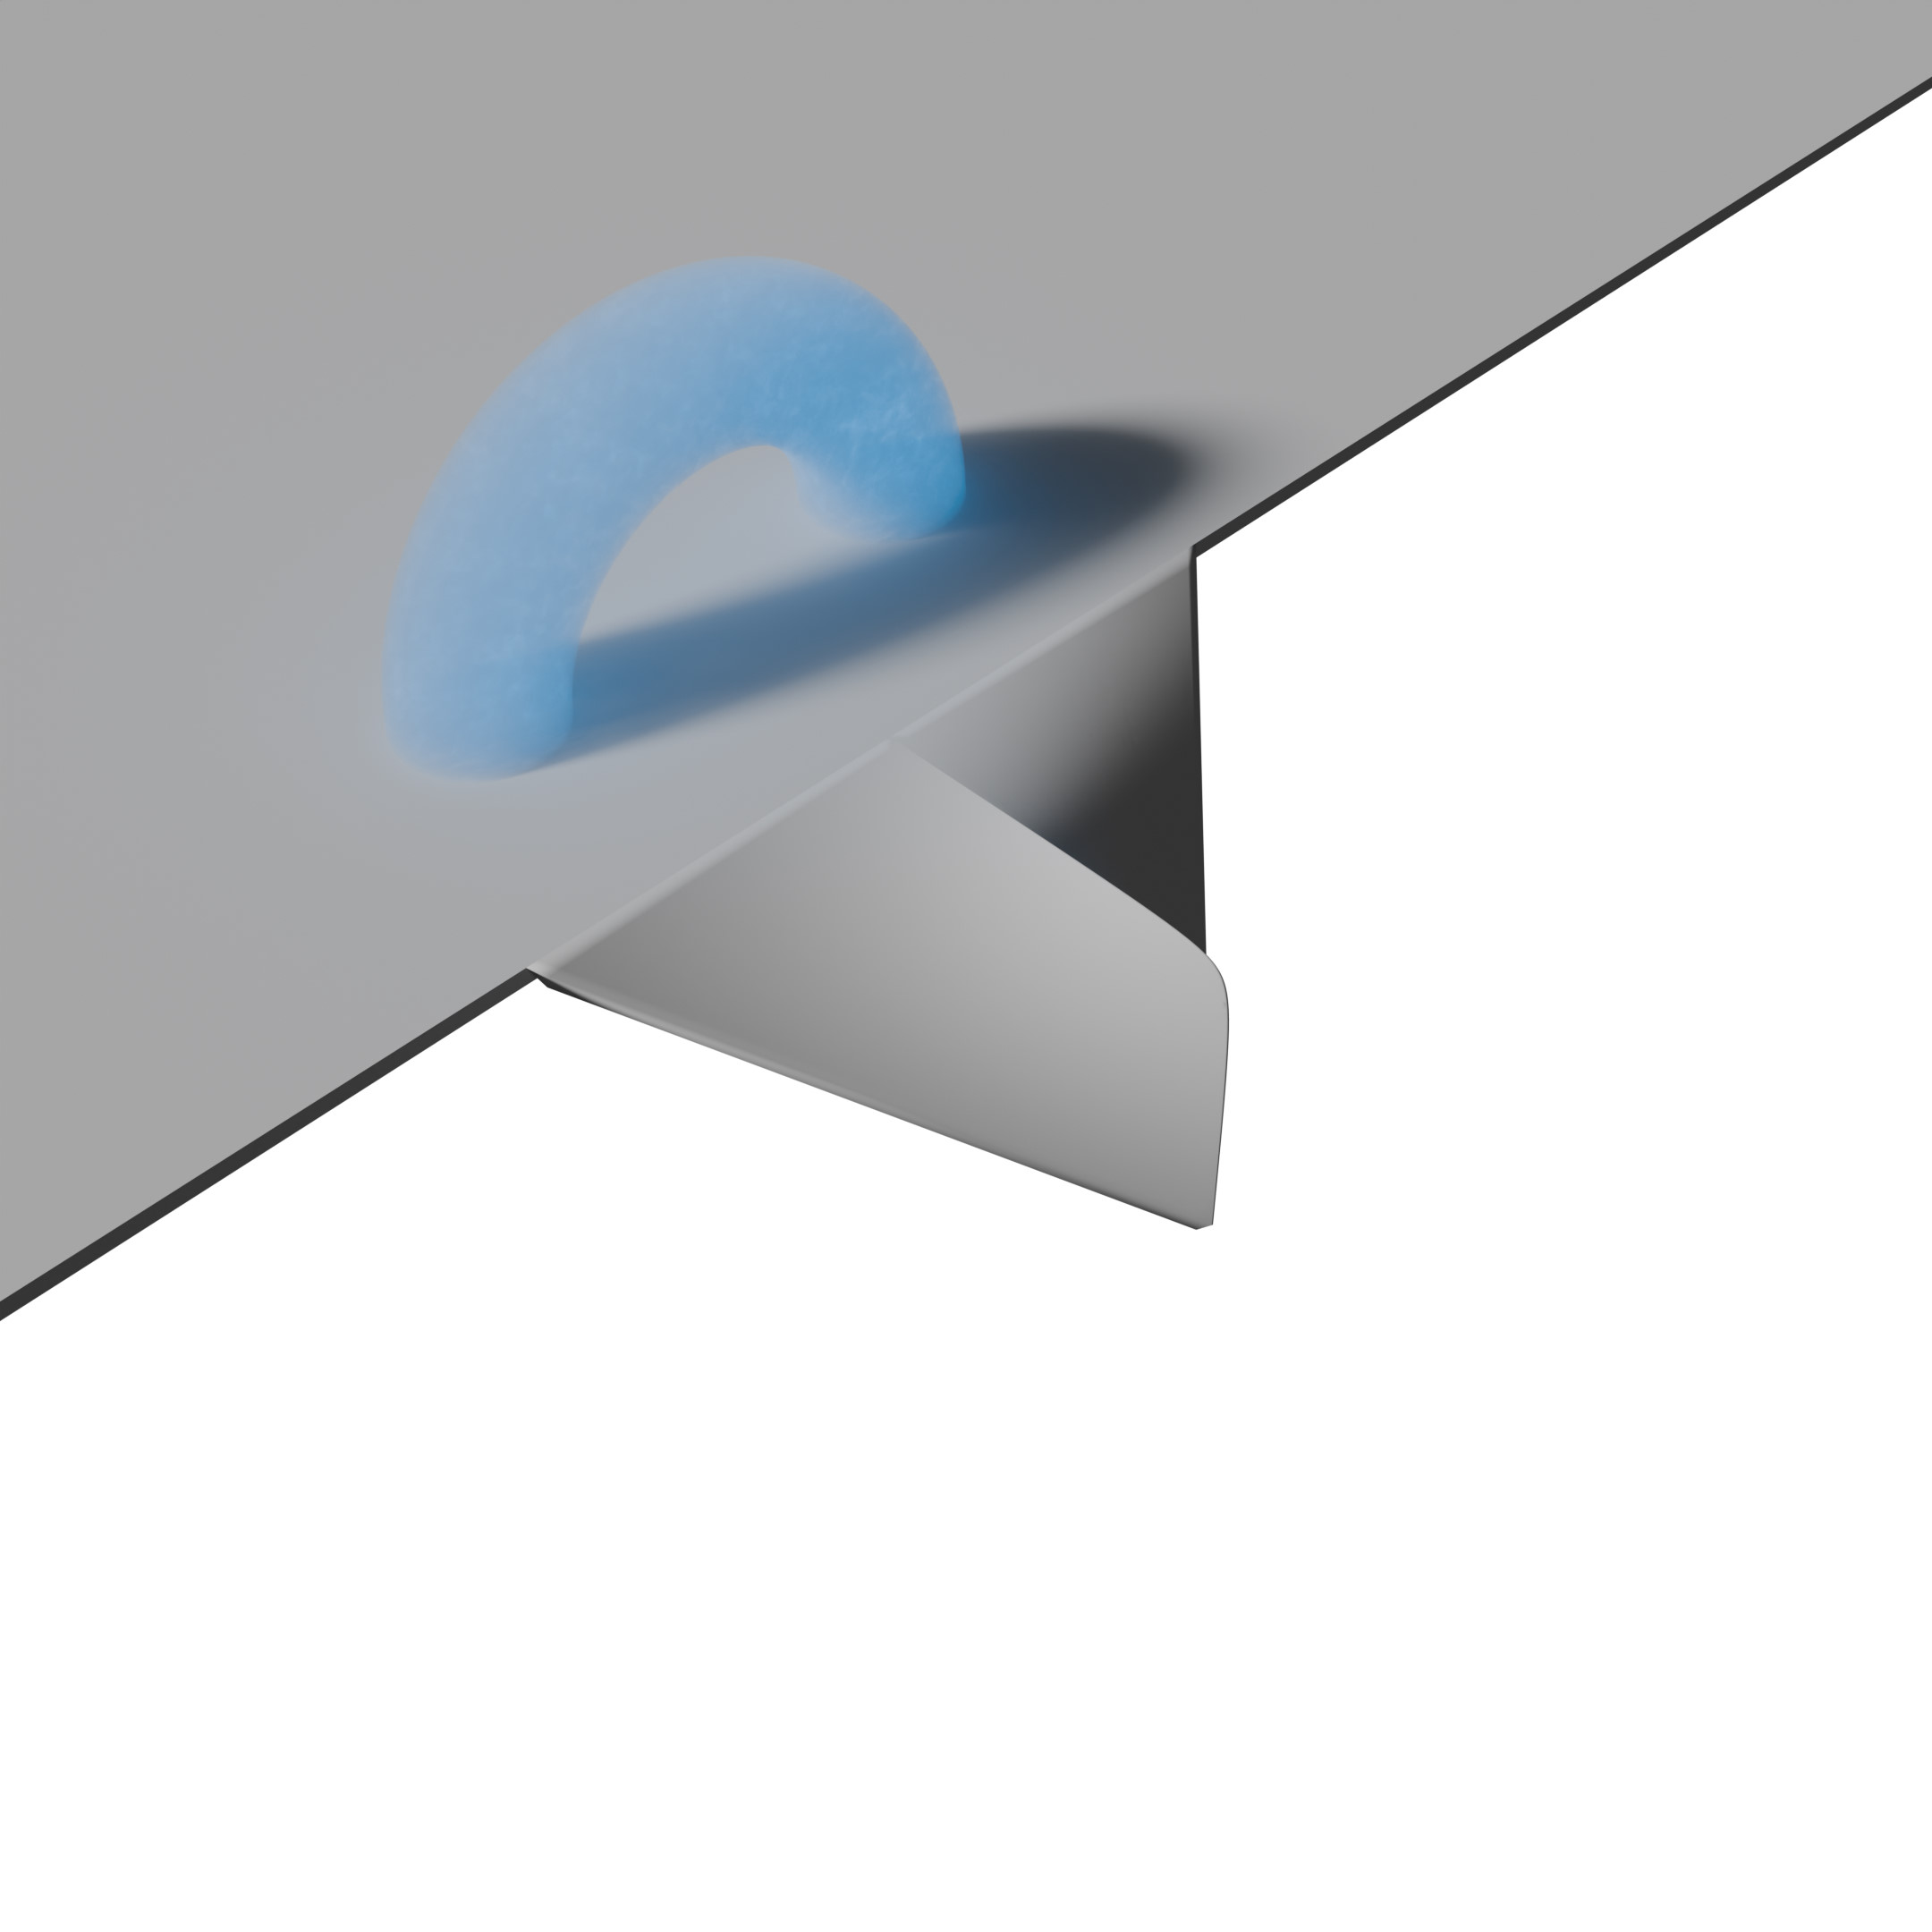
\includegraphics[width=0.3\textwidth]{papers/wirbelringe/fig/versuch_moment_3.jpg}
    }
    \caption{3D Darstellung in Blender des gewünschten Versuchsausgangs.}
    \label{Wirbelringe:fig:wirbelringversuch}
\end{figure}


\begin{enumerate}
    \item Abbildung \ref{Wirbelringe:fig:versuch_moment_1}: Ein Wirbelring wird auf eine Kante gerichtet erzeugt
    \item Abbildung \ref{Wirbelringe:fig:versuch_moment_2}: Dieser Wirbelring trifft auf die Kante und übernimmt diese als neue Grenzflächen da diese etwa parallel zu der vorherigen waren.
    \item Abbildung \ref{Wirbelringe:fig:versuch_moment_3}: Durch leichten Änderungen können sich die Grenzflächen aus der vertikalen in die horizontale Ebene ändern.
    Somit können diese auf eine andere Fläche übergehen.
    Der Wirbelring kann sich so weiter fortbewegen.
\end{enumerate}
    
